\chapter{Classificação utilizando aprendizado profundo}

O capítulo anterior tratou-se de uma solução baseada em seleção de candidatos, extração de características e posterior classificação, o que caracteriza uma técnica superficial. Nesse capítulo propomos uma solução híbrida, que utiliza a seleção de candidatos idêntica à anterior, porém utiliza técnicas profundas de classificação de modo que os candidatos são diretamente inseridos no classificador. Inicialmente introduz-se as redes MLP e convolucionais, fornecendo as bases teóricas, funções de ativação e processo treinamento.  Questões relativas à implementação também são abordadas.

\section{Perceptron Multicamadas (MLP)}

Segundo \cite{DLbook}, uma rede de perceptrons multicamadas (MLP) também pode ser chamada de rede profunda sem realimentação (\textit{deep feedforward networks}), também chamada de rede neural, e tem como objetivo aproximar uma função $f^*$. Para o problema de classificação, $y=f^*(x)$, onde $y$ é a categoria e $x$ a amostra, a rede define um mapeamento $y = f(x,\theta)$, onde $\theta$ são os parâmetros do modelo. O problema consiste em encontrar $\theta$ que resulte na melhor aproximação de $f^*$.

Essa estrutura é chamada de rede pois são representadas como um conjunto de camadas, cada uma alimentando a próxima, o que gera uma cadeia de funções: $y=f^1(f^2(f^3(x)))$, cada qual representando uma camada. Além disso, não ocorre alimentação pois a informação flui continuamente através das camadas desde a entrada $x$ sequencialmente até a camada de saída $y$.

Parte-se de um modelo linear simples,
\begin{equation}
y=w^Tx+b
\end{equation}
em que $w$ corresponde ao vetor de pesos do classificador e $b$ bias. Verifica-se que esse modelo pode ser treinado de maneira simples e rápida, porém serve apenas para casos em que o dataset é linearmente separável, diferente da maioria dos problemas reais. Como visto na seção \ref{sec:classificacao:svm}, técnicas de mapeamento não lineares $\phi(x)$ são alternativas para tentar tornar essas amostras linearmente separáveis, como é o caso da função RBF. Na abordagem superficial, deve-se escolher esse mapeamento de maneira específica às amostras de forma manual. 

Advém, então, uma das principais contribuições dos métodos profundos: a função de mapeamento $\phi(x,\theta)$ é determinada, entre uma gama ampla de funções, pelo próprio sistema através dos parâmetros $\theta$. Isso pode ser interpretado como a seleção automática, pelo algoritmo, do extrator de características que melhor represente o dataset. Assim, o modelo se torna 
\begin{equation}
y=f(x,\theta,w) = w^T\phi(x,\theta)
\end{equation}
Na rede, $\phi$ corresponde às camadas intermediárias. Os parâmetros $w$ mapeiam, então, o resultado da camada intermediária $\phi(x,\theta)$, que representam as descrições da amostra, para a camada de saída $y$. O princípio de aprender o extrator características mais apropriado para o dataset não é exclusivo para redes MLP e se aplica a outros modelos de aprendizado profundo.

Nota-se, ainda, que no caso mais geral, para camadas de saída com funções de ativação não lineares, teríamos o modelo generalizado
\begin{equation}
y=f(x,\theta,w) = \gama(w^T\phi(x,\theta)+b)
\end{equation}
onde $\gama(x)$ é a função de ativação da camada de saída.

\section{Funções de ativação}
Como visto na seção \ref{introducao:perceptron}, os perceptrons aplicam uma função de ativação ao somatório ponderado das entradas. A escolha dessa função está associada à interpretação que se dá à saída. Duas funções foram utilizadas nesse trabalho e serão introduzidas a seguir.

\subsection{Sigmoide}
Como visto anteriormente, a escolha da função relaciona-se com a interpretação do valor de saída. Para classificadores interpreta-se o valor dos perceptrons da camada de saída como probabilidades da amostra pertencer a uma determinada classe. Nesse caso espera-se que esses valores estejam no intervalo $[0,1]$. Uma função que assegura essa condição é a sigmoide
\begin{equation}
	\label{eq:sigm}
	\sigma(x) = \frac{1}{1+e^{-x}}
\end{equation}

\begin{figure}[h]
\centering
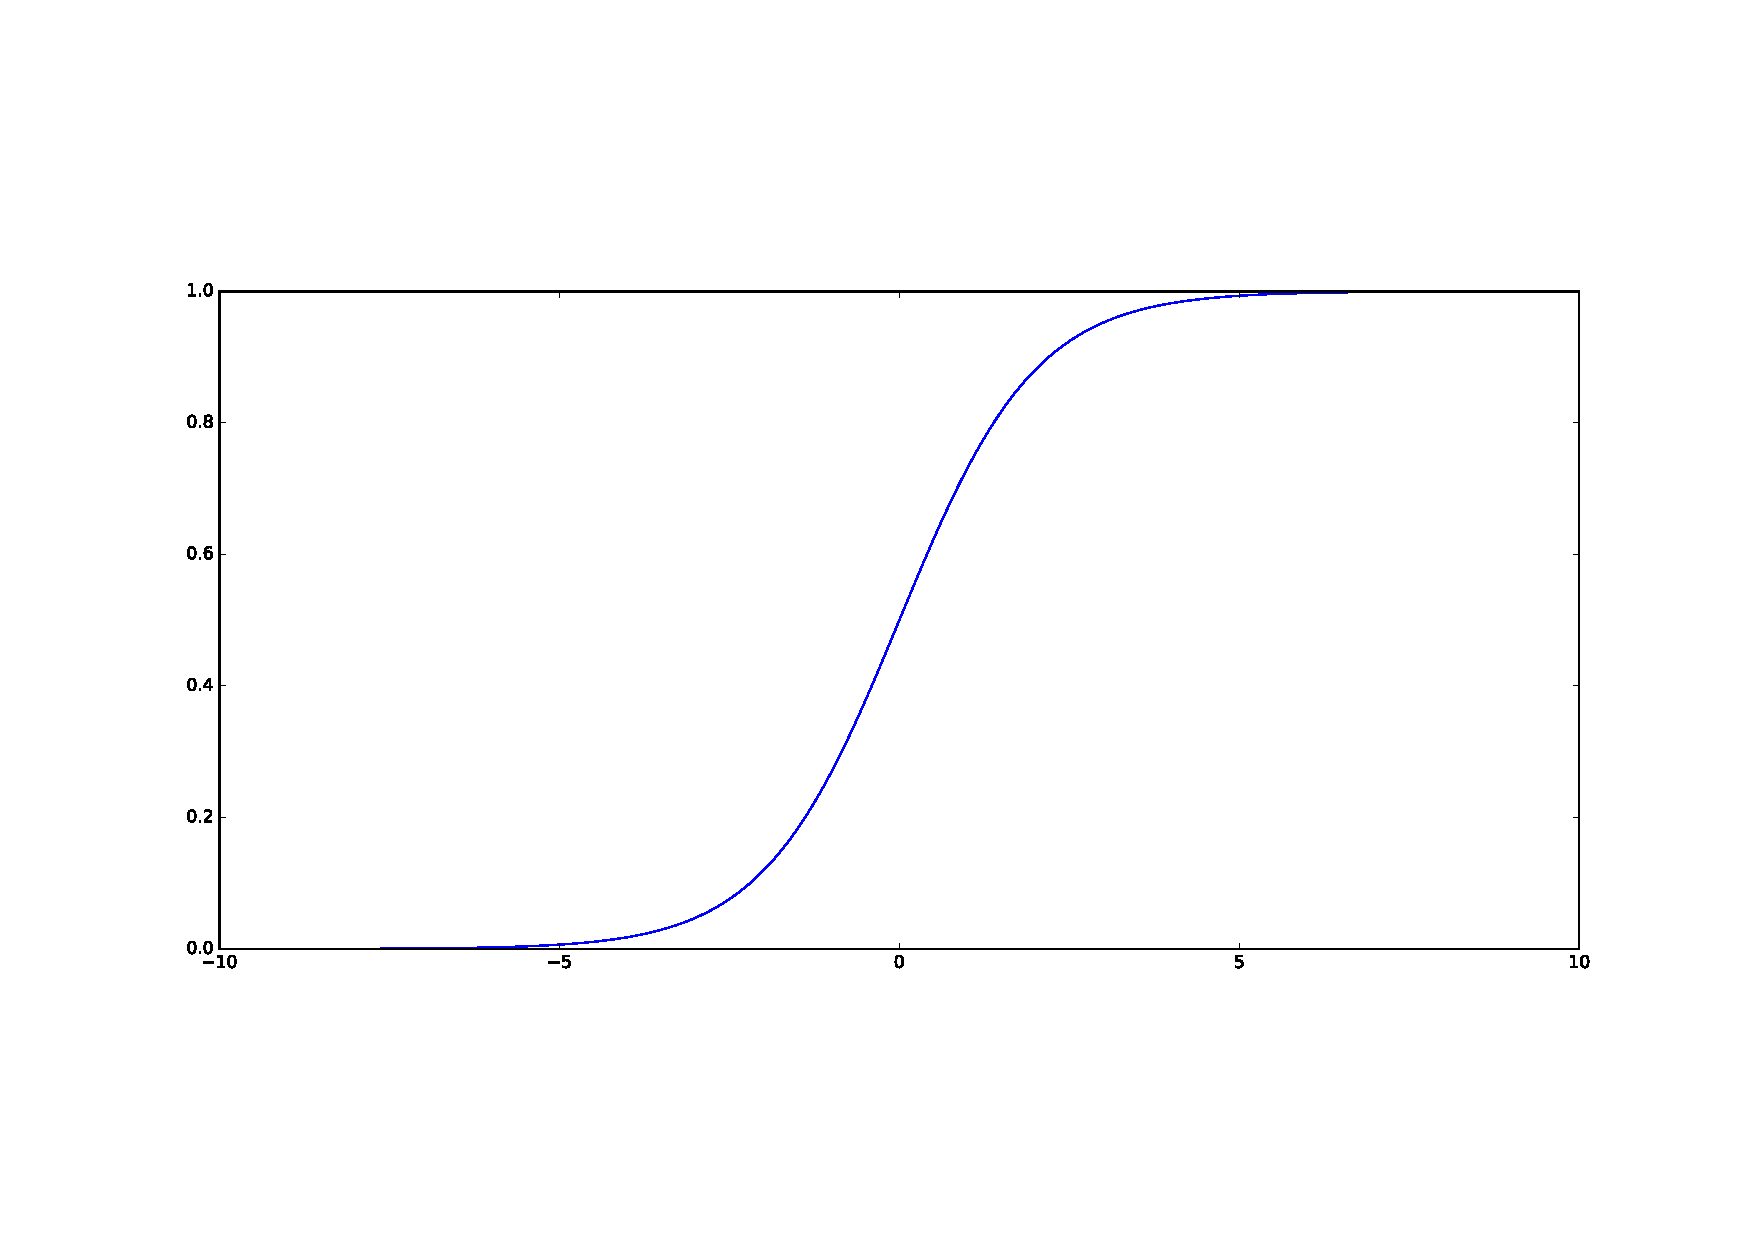
\includegraphics[width=0.9\textwidth]{deep/sigmoid}
\caption{Gráfico mostrando o comportamento da sigmoide}
\label{fig:sigmoid}
\end{figure}

Outra característica importante é a não linearidade da função que permite transformar conjuntos não linearmente separáveis. Por outro lado, observa-se que essa função satura facilmente com entradas pŕoximas de 1 ou 0, ocasionando uma derivada praticamente nula nessas regiões. Como será visto adiante isso é um problema ao se considerar que a derivada dessa função definirá a atualização dos pesos desses perceptrons durante o processo de treinamento. Ao propagar esse processo camada a camada, verificam-se derivadas cada vez menores, o que causa o problema do gradiente enfraquecido, em que as camadas iniciais não conseguem aprender pois o gradiente é muito reduzido.

\subsection{RELU}
Para resolver o problema do gradiente enfraquecido a \textit{Rectified Linear Unit -- RELU} foi proposta \cite{nair2010relu} como
\begin{equation}
	\label{eq:relu}
	\text{RELU}(x) = \max\{0,x\}
\end{equation}

Observa-se que para valores positivos essa função tem uma derivada constante e igual a um, proporcionando uma taxa de aprendizado considerável sempre que o perceptron estiver ativo. Por outro lado, para valores negativos considera-se o perceptron inativo e os pesos não são atualizados. Ao mesmo tempo essa característica garante a não linearidade da função.

\section{Treinamento}
%utilizar referencia http://neuralnetworksanddeeplearning.com/chap3.html#the_cross-entropy_cost_function
O processo de treinamento de uma rede neural é um problema de otimização. Porém, diferentemente do caso do SVM, trata-se de uma otimização não convexa, isto é, existem múltiplos mínimos locais para a função custo e diversas soluções podem ser encontradas, dependendo dos valores iniciais dos parâmtros. Esse fato advém do caráter não linear das funções de ativação nas camadas intermediárias que irão definir a extração de características.

Durante essa etapa otimiza-se os parâmetros $\theta$ de forma que $y \approx f^*(x)$. Isso é feito através da minimização de uma função custo $J(\theta)$, que mede a proximidade entre os resultados do modelo e o conjunto de treinamento. Em geral escolhe-se a função de entropia cruzada
\begin{equation}
J(\theta) = -E_{x,y \sim p_{data}}\log p_\text{model}(y|x)
\end{equation}
A escolha da função custo está associada também à função de ativação das camadas de saída. Isso é importante pois no caso de uma ativação sigmoide a saída satura rapidamente, o que provoca uma derivada muito pequena que ocasionará um gradiente desprezível e consequentemente pouca variação nos pesos dos perceptrons. Essa formulação dá um caráter mais geral 

Observa-se que a camada de saída possui um valor alvo bem definido, porém as camadas intermediárias (\textit{hidden layers}) não têm um comportamento diretamente especificado. Nesse caso, utiliza-se o algoritmo de propagação reversa de erros (\textit{back-propagation}) para terminar como as variações dos pesos dos perceptrons devem se propagar pela rede.


\section{Redes convolucionais}

\section{Implementação}
Keras e theano. Diferentes configurações.
